% !TEX program = xelatex
\documentclass[conference,a4paper]{IEEEtran}
\usepackage{fontspec}
\setmainfont{TeX Gyre Termes}
\usepackage{amsmath,amssymb,graphicx,booktabs,tabularx,multirow}
\usepackage{float,adjustbox,tikz,pgfplots}
\usetikzlibrary{arrows.meta,positioning,calc}
\pgfplotsset{compat=1.18}
\definecolor{inkblue}{HTML}{193C65}
\definecolor{mutedblue}{HTML}{EAF1F7}
\definecolor{cgreen}{HTML}{296B53}
\definecolor{cred}{HTML}{9D4D45}
\usepackage{xurl}
\usepackage[hidelinks]{hyperref}
\usepackage[backend=biber,style=ieee,sorting=none,maxbibnames=4]{biblatex}
\addbibresource{ref.bib}
\graphicspath{{./}{../../latex_report_source/}{../pvsg-trd-m5-v1/}}
\newcommand{\nd}{\textemdash}
\newcommand{\srcnote}[1]{\par\smallskip{\raggedright\footnotesize #1\par}\smallskip}
\newcommand{\reporttodo}[2]{\par\smallskip\noindent\textit{Bằng chứng còn thiếu (#1).} #2\par}
\renewcommand{\tablename}{Bảng}
\renewcommand{\figurename}{Hình}
\renewcommand{\abstractname}{Tóm tắt}
\renewcommand{\IEEEkeywordsname}{Từ khóa}
\renewcommand{\appendixname}{Phụ lục}
\title{Biểu diễn đồ thị ngữ nghĩa cho chỉnh sửa ảnh\\và dự đoán quan hệ trong video}
\author{\IEEEauthorblockN{Hồ Thanh Bình, Dương Thuỷ Tiên, Bùi Mạnh Hùng, Nguyễn Đăng Khoa, Nguyễn Đăng Thới Toàn}
\IEEEauthorblockA{Khoa Công nghệ Thông tin, Trường Đại học Khoa học Tự nhiên, ĐHQG-HCM\\
Học máy với dữ liệu đồ thị, 2026\\
Giảng viên hướng dẫn: PGS. TS. Lê Ngọc Thành và ThS. Huỳnh Lâm Hải Đăng}}
\begin{document}
\maketitle
\begin{abstract}
Đồ án dùng đồ thị cảnh để trả lời ba câu hỏi: quan hệ nào tồn tại giữa hai đối tượng,
cần sửa thành phần nào của đồ thị theo câu lệnh và ảnh sau chỉnh sửa có giữ đúng
nội dung yêu cầu hay không. Trên VG150, GAT tăng 1,65 điểm phần trăm mR@50 so
với MLP. Điều chỉnh hàm mất mát theo tần suất lớp tăng 6,48 điểm khi tắt tri thức
nền. Ở bài toán biến đổi đồ thị, GNN đạt micro-F1 7,34\% trên MagicBrush và
82,44\% trên bộ cặp đồ thị có cấu trúc EMNLP 2020. Trên 200 yêu cầu chỉnh sửa ảnh,
điểm nhất quán đồ thị đánh giá được 45,5\% số cặp, với tương quan Spearman 0,1767
so với nhãn người trên tập có điểm. Phần mở rộng video kiểm tra dự đoán quan hệ
và thời gian trên track chuẩn của PVSG. Trong tám cấu hình, Temporal Conv đạt
R@50 cao nhất (8,63\%), còn ST-GAT đạt mR@50 cao nhất (2,38\%).
\end{abstract}
\begin{IEEEkeywords}
đồ thị cảnh, dự đoán quan hệ, chỉnh sửa đồ thị, nhất quán ngữ nghĩa, quan hệ theo thời gian
\end{IEEEkeywords}
\section{Giới thiệu}
Một yêu cầu như “thêm con mèo dưới gốc cây” xác định cả đối tượng cần thêm, vị trí tương đối và phần cảnh cần giữ. Đồ thị cảnh biểu diễn hai đối tượng bằng đỉnh và quan hệ có hướng bằng cạnh. Đồ án chọn nhánh ảnh tĩnh làm bài toán chính. Các mô hình thị giác và sinh ảnh được dùng ở chế độ
đóng băng; phần học là các mô hình trên đồ thị. Bảng~\ref{tab:scorecard} tổng hợp
kết quả trước khi đi vào thiết lập, đối chứng và phân tích lỗi.

\begin{table*}[!t]\centering\small
\caption{Kết quả chính của ba nhiệm vụ và thực nghiệm mở rộng. Các hàng khác dataset, split hoặc metric không dùng để xếp hạng chung.}\label{tab:scorecard}
\begin{tabularx}{\linewidth}{@{}p{10mm}p{28mm}p{29mm}X@{}}
\toprule NV & Phần & Dữ liệu / split & Kết quả chính\\\midrule
1 & Relation prediction & VG150 / test & GAT mR@50 \textbf{18,61\%}; hơn MLP \textbf{1,65 pp}.\\
1 & Loss ablation & VG150 / test & Adjusted, KG-off: mR@50 \textbf{24,59\%}, tăng \textbf{6,48 pp} so CE-off.\\
1 & KG fusion & VG150 / test & Pair-real mR@50 \textbf{25,24\%}; hơn shuffled 0,24 pp, chỉ 2/3 seed tăng.\\
2A & Phương pháp 2023+ & Custom GQA / test & PE-PLPR mR@50 \textbf{4,07\%}.\\
2A & AlignG ablation & Custom GQA / test & GC mR@50: \textbf{4,07 $\to$ 4,62\%}; bản adapted.\\
2B & Biến đổi đồ thị gốc & MagicBrush / test & GNN micro-F1 \textbf{7,34\%}; exact target graph \textbf{0\%}.\\
2B & Dataset thay thế & EMNLP 2020 / test & GNN micro-F1 \textbf{82,44\%}; macro-F1 \textbf{55,03\%}.\\
3 & Nhất quán đồ thị & VN100 / 200 edit & $\rho_G=\mathbf{0,1767}$; coverage \textbf{45,5\%}.\\
3 & Baseline ảnh & Tập giao $N=91$ & $-\mathrm{LPIPS}$ 0,1962; Graph 0,1767; CLIPScore 0,0561.\\
Video & Quan hệ video & PVSG / test & Conv kernel 5 đạt R@50 \textbf{8,63\%}; ST-GAT đạt mR@50 \textbf{2,38\%} trên track chuẩn.\\
\bottomrule\end{tabularx}
\end{table*}

\subsection{Quy ước đọc kết quả}
R và mR là phần trăm; pp là \emph{điểm phần trăm}, không phải phần trăm tăng
tương đối. Mean $\pm$ std là trung bình và độ lệch chuẩn mẫu qua ba seed,
không phải khoảng tin cậy. GC (graph constraint) giữ một predicate cho mỗi cặp
object có hướng; NG cho phép nhiều predicate. Bảng VG150 chính dùng GC
reference-v1 trên 26.446 ảnh test. Long-tail và zero-shot cũng đã bổ sung
kết quả test; custom GQA có cả tập validation và tập test của đồ án. Các ca định tính VG150 dùng validation.

\subsection{Ba kết luận cần kiểm chứng}
\begin{enumerate}
\item \textbf{Nhiệm vụ 1:} GAT có lợi so với MLP, nhưng điều chỉnh loss
tác động tới mR lớn hơn các cách thêm KG đã thử. Tăng mR không đồng nghĩa tăng R.
\item \textbf{Nhiệm vụ 2:} phương pháp mới tăng mR trên custom GQA; học graph operation
khả thi hơn khi supervision có cấu trúc. EMNLP không thay thế bằng chứng còn thiếu
của pipeline từ ảnh MagicBrush.
\item \textbf{Nhiệm vụ 3:} điểm đồ thị cung cấp chẩn đoán theo object/quan hệ nhưng
độ phủ thấp. Tương quan hiện tại chưa chứng minh ưu thế so với baseline ảnh.
\end{enumerate}
\srcnote{Nguồn số liệu: các report versioned trong \path{reports/level1}, \path{reports/level2}
và \path{docs/LEVEL3_RESULTS_V1.md}. Ánh xạ chi tiết nằm trong \path{SOURCE_MAP.md} đi kèm.}


\section{Nhiệm vụ 1 -- VG150: dự đoán quan hệ và tri thức nền}
\subsection{Thiết lập PredCls và mô hình}
Đầu vào là ảnh, hộp và nhãn object GT; đầu ra là predicate cho cặp object có
hướng. Không dự đoán lại object và không đưa cạnh quan hệ GT vào graph message
passing. VG150 là tập con của Visual Genome~\cite{krishna2017visualgenome}.

\begin{table}[!ht]\centering\small
\caption{Thiết lập thực nghiệm VG150.}\label{tab:vgsetup}
\begin{tabularx}{\linewidth}{@{}p{23mm}X@{}}\toprule
Thành phần & Cấu hình\\\midrule
Split, vocabulary & Train 57.723 / val 5.000 / test 26.446 ảnh; 150 object, 50 predicate và background.\\
Đặc trưng object & CLIP ViT-B/32 đóng băng, 512 chiều; hình học 5 chiều; label embedding học được 32 chiều.\\
MLP / GAT & MLP phân lớp cặp, không message passing; GAT 2 lớp, 4 heads, hidden 256, dropout 0,1.\\
Graph đầu vào & Cạnh có hướng giữa các object; edges-off bỏ cạnh giữa các object, vẫn giữ self-loop.\\
KG & Embedding 64 chiều và bit liên kết hợp lệ; WordNet 150/150, ConceptNet 138/150 lớp object.\\
Tối ưu & AdamW, learning rate $10^{-3}$, weight decay $10^{-2}$; effective batch 512, negative ratio 3.\\
Dừng và seed & Tối đa 200 epoch, patience 15; seed 42, 123, 3407. Giữ checkpoint đã chọn từ validation.\\
Đánh giá cuối & 18 cấu hình $\times$ 3 seed = 54 checkpoint; inference batch 128, cùng test và evaluator reference-v1.\\
\bottomrule\end{tabularx}\end{table}

Với object $i$, đặc trưng là $x_i=[v_i;b_i;e(c_i);k_i;m_i]$,
trong đó $k_i$ và $m_i$ chỉ có ở nhánh KG. GAT~\cite{velickovic2018gat} tính
\[
h_i^{(\ell+1)}=\mathop{\Vert}_{a=1}^{H}
\sigma\!\left(\sum_{j\in\mathcal N(i)}\alpha_{ij}^{(\ell,a)}
W^{(\ell,a)}h_j^{(\ell)}\right).
\]
\[
z_{ij}=f_\theta(h_i,h_j,\text{đặc trưng cặp}).
\]
MLP không tổng hợp hàng xóm. KG lấy từ
WordNet/ConceptNet~\cite{miller1995wordnet,speer2017conceptnet}, nhúng bằng
TransE, RotatE hoặc ComplEx~\cite{bordes2013transe,sun2019rotate,trouillon2016complex};
không lấy quan hệ test để xây KG.

\subsection{Protocol và kiểm soát so sánh}
Reference-v1 khớp đúng predicate, lớp subject/object và IoU của cả hai hộp
ít nhất 0,5. R@K là trung bình recall theo ảnh; mR@K tính recall theo ảnh
cho từng predicate rồi trung bình trên 50 lớp. GT trùng được giữ khi chấm.
Trong train, sampler bỏ cặp có nhiều predicate khác nhau; cần lưu ý khác biệt
giữa supervision huấn luyện và GT đánh giá khi đọc lỗi đa nhãn.

Hai đợt inference gồm 27 checkpoint gốc và 27 checkpoint loss/fusion.
Checkpoint và source được khóa, không chọn lại theo test hay evaluator mới.
Các thiết kế cải tiến dựa trên train/validation. Test đã từng được dùng ở các
vòng trước nên không mô tả đây là holdout chưa từng xem; cũng không suy từ
thứ tự thời gian rằng thiết kế loss đã được tinh chỉnh theo test.
\srcnote{Nguồn: \path{docs/evaluation/PredCls.md};
\path{reports/level1/reference-test27-v1/} và
\path{reference-loss-fusion-test27-v1/}.}


\subsection{MLP, GAT và KG: bảng test chính}
\begin{table*}[!t]\centering\small
\caption{VG150 test, GC reference-v1; mean $\pm$ sample std (\%), ba seed.}\label{tab:vgmain}
\begin{tabular}{@{}lrrrr@{}}\toprule
Cấu hình & R@50 & R@100 & mR@50 & mR@100\\\midrule
MLP & $63,56\pm0,77$ & $66,40\pm0,29$ & $16,95\pm1,52$ & $19,52\pm1,42$\\
GAT & $63,87\pm0,73$ & $66,21\pm0,70$ & $\mathbf{18,61\pm0,25}$ & $\mathbf{20,95\pm0,21}$\\
KG-off & $63,89\pm0,38$ & $66,24\pm0,30$ & $18,44\pm0,29$ & $20,72\pm0,43$\\
WordNet--TransE & $64,15\pm0,29$ & $66,69\pm0,34$ & $17,84\pm0,09$ & $20,34\pm0,08$\\
WordNet edges-off & $64,11\pm1,15$ & $66,46\pm1,13$ & $18,41\pm0,90$ & $20,72\pm0,76$\\
ConceptNet--TransE & $64,10\pm0,27$ & $66,45\pm0,28$ & $18,39\pm0,29$ & $20,71\pm0,28$\\
ConceptNet edges-off & $\mathbf{64,59\pm0,19}$ & $\mathbf{66,97\pm0,16}$ & $18,15\pm0,28$ & $20,47\pm0,32$\\
ConceptNet--RotatE & $64,21\pm0,37$ & $66,60\pm0,46$ & $18,57\pm0,42$ & $20,93\pm0,35$\\
ConceptNet--ComplEx & $64,37\pm0,18$ & $66,79\pm0,25$ & $18,33\pm0,24$ & $20,75\pm0,18$\\
\bottomrule\end{tabular}\end{table*}

GAT tăng \textbf{1,65 pp mR@50} so với MLP, cùng dấu ở cả ba seed
($+0,970/+3,131/+0,861$ pp). Tuy nhiên R@100 giảm 0,19 pp.
Các nhánh ghép KG tại node chưa vượt GAT về mean mR@50.
WordNet--TransE thấp hơn KG-off 0,60 pp; RotatE gần GAT ($-0,04$ pp),
với một seed giảm.

Edges-off ở WordNet và ConceptNet cho R cao hơn hoặc gần bản có cạnh:
message passing không có lợi ở mọi nhánh. GAT và KG-off là các cấu hình/checkpoint
riêng; không coi các hàng là một checkpoint bật/tắt lúc inference.

\subsection{Adjusted loss: tác động lớn hơn KG}
Dùng prior $p_c$ tính từ train với add-one smoothing:
\[
\mathcal L_{\mathrm{adj}}
=\operatorname{CE}\!\left(z+\tau\log p_{\mathrm{train}},y\right),
\qquad \tau=0,25.
\]
Phần cộng prior chỉ áp dụng khi train; inference dùng logits gốc $z$.
Bốn cấu hình tạo đối chứng chéo giữa loss và KG.

\begin{table*}[!t]\centering\small
\caption{Loss ablation trên VG150 test. Baseline riêng, không trộn với bảng~\ref{tab:vgmain}.}\label{tab:loss}
\begin{tabular}{@{}lrrrr@{}}\toprule
Cấu hình & R@50 & R@100 & mR@50 & mR@100\\\midrule
CE, KG-off & $64,42\pm0,10$ & $66,85\pm0,09$ & $18,11\pm0,16$ & $20,56\pm0,19$\\
CE, KG-on & $63,63\pm0,14$ & $65,93\pm0,13$ & $19,27\pm0,75$ & $21,51\pm0,91$\\
Adjusted, KG-off & $62,18\pm0,16$ & $64,81\pm0,13$ & $24,59\pm0,93$ & $27,89\pm1,02$\\
Adjusted, KG-on & $62,01\pm0,31$ & $64,71\pm0,46$ & $24,67\pm1,07$ & $28,00\pm1,19$\\
\bottomrule\end{tabular}\end{table*}

Giữ KG-off, adjusted tăng \textbf{6,48 pp mR@50} nhưng giảm
\textbf{2,24 pp R@50}. Với KG-on, mR tăng 5,40 pp.
Thêm KG vào adjusted chỉ tăng 0,09 pp mR@50 và có seed giảm 2,09 pp:
lợi ích chính đến từ loss, chưa có bằng chứng về lợi ích KG cộng thêm ổn định.


\subsection{Fusion và shuffled-KG: kiểm tra nguồn lợi ích}
Pair fusion đưa embedding tri thức của cặp object vào nhánh dự đoán quan hệ;
visual fusion dùng nhánh hợp nhất có điều kiện theo thông tin thị giác.
Shuffled-KG giữ cơ chế hợp nhất nhưng xáo trộn ánh xạ embedding--nhãn object,
kiểm tra phần tăng điểm có gắn với nội dung tri thức hay không.
Các nhánh dùng adjusted loss và baseline riêng của cohort fusion.

\begin{table*}[!t]\centering\small
\caption{Fusion trên VG150 test; shuffled là một permutation cố định.}\label{tab:fusion}
\begin{tabular}{@{}lrrrr@{}}\toprule
Cấu hình & R@50 & R@100 & mR@50 & mR@100\\\midrule
Fusion baseline & $62,06\pm0,39$ & $64,83\pm0,21$ & $24,32\pm0,91$ & $27,72\pm1,08$\\
Pair, KG thật & $62,37\pm0,19$ & $65,01\pm0,20$ & $\mathbf{25,24\pm0,39}$ & $\mathbf{28,65\pm0,27}$\\
Pair, shuffled & $62,34\pm0,18$ & $65,06\pm0,24$ & $25,00\pm0,71$ & $28,33\pm0,74$\\
Visual, KG thật & $62,34\pm0,21$ & $65,05\pm0,22$ & $24,52\pm0,64$ & $27,98\pm0,73$\\
Visual, shuffled & $62,20\pm0,23$ & $64,96\pm0,22$ & $24,82\pm1,25$ & $27,94\pm1,10$\\
\bottomrule\end{tabular}\end{table*}

\begin{table}[!ht]\centering\small
\caption{Delta mR@50 ghép cặp cùng seed trên test; pp, tính trước khi làm tròn.}
\begin{adjustbox}{max width=\linewidth}\begin{tabular}{@{}lrrrr@{}}\toprule
Treatment $-$ control & Mean & Seed 42 & Seed 123 & Seed 3407\\\midrule
Adjusted-off $-$ CE-off & +6,479 & +6,081 & +7,710 & +5,645\\
Adjusted-on $-$ Adjusted-off & +0,086 & +0,557 & $-2,090$ & +1,793\\
Pair-real $-$ fusion baseline & +0,926 & +1,783 & $-0,560$ & +1,556\\
Pair-real $-$ pair-shuffled & +0,238 & +0,400 & $-0,823$ & +1,135\\
Visual-real $-$ visual-shuffled & $-0,300$ & $-0,917$ & +0,752 & $-0,735$\\
\bottomrule\end{tabular}\end{adjustbox}\end{table}

\begin{figure}[!ht]\centering
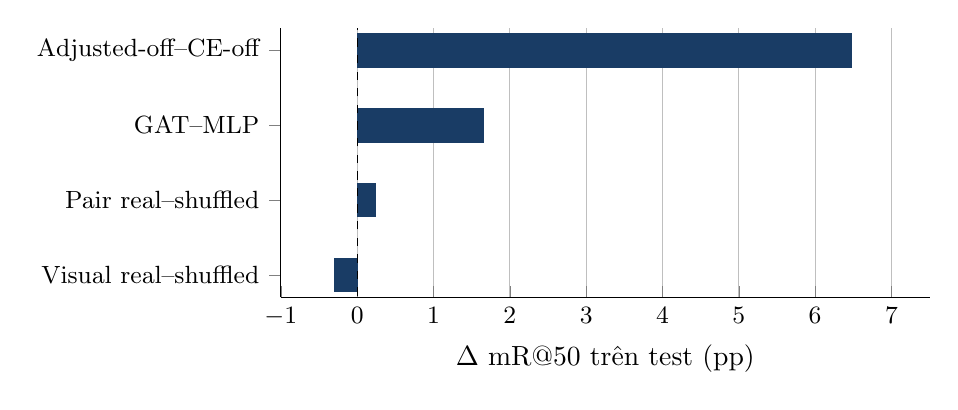
\begin{tikzpicture}
\begin{axis}[width=.81\linewidth,height=5.0cm,xbar,xmin=-1,xmax=7.5,
ytick={1,2,3,4},yticklabels={Visual real--shuffled,Pair real--shuffled,GAT--MLP,Adjusted-off--CE-off},
xlabel={$\Delta$ mR@50 trên test (pp)},tick label style={font=\small},
axis x line*=bottom,axis y line*=left,xmajorgrids,bar width=12pt]
\addplot[fill=inkblue,draw=inkblue] coordinates {(-.300,1) (.238,2) (1.654,3) (6.479,4)};
\draw[dashed] (axis cs:0,.5)--(axis cs:0,4.5);
\end{axis}\end{tikzpicture}
\caption{Độ lớn tác động của các đối chứng. Mỗi thanh thuộc cohort riêng;
delta trung bình là thống kê mô tả, không phải kiểm định ý nghĩa thống kê.}
\end{figure}

Pair-real có mean mR@50 cao nhất trong 18 cấu hình, nhưng hơn shuffled
chỉ 0,24 pp và thua ở seed 123. Visual-real thấp hơn shuffled trung bình.
\textbf{Chưa quy toàn bộ lợi ích fusion cho nội dung KG};
ba seed và một permutation chưa đủ để khẳng định khác biệt nhỏ là ổn định.
\srcnote{Nguồn: \path{reference-loss-fusion-test27-v1/analysis.json} và \path{tables.md}.}


\subsection{Long-tail và zero-shot: kết quả test}
Long-tail dùng \textbf{26.446 ảnh test} của 54 checkpoint; tính trên CPU từ
recall từng predicate đã lưu, không inference lại.
Head/body/tail giữ nguyên theo tần suất train: 10/20/20 predicate,
chiếm 88,40/10,14/1,46\% annotation train. Top-K vẫn lấy trên toàn ảnh.

\begin{table}[!ht]\centering\small
\caption{Long-tail test: GC mR@50 (\%), mean $\pm$ sample std ba seed.}\label{tab:tail}
\begin{adjustbox}{max width=\linewidth}\begin{tabular}{@{}lrrr@{}}\toprule
Cấu hình & Head (10 lớp) & Body (20 lớp) & Tail (20 lớp)\\\midrule
MLP & $49,93\pm1,58$ & $14,12\pm2,14$ & $3,29\pm0,87$\\
GAT & $51,03\pm0,69$ & $16,88\pm0,99$ & $4,12\pm0,08$\\
CE, KG-off & $51,10\pm0,15$ & $16,19\pm0,41$ & $3,54\pm0,20$\\
Adjusted, KG-off & $50,72\pm0,10$ & $26,56\pm0,94$ & $9,55\pm1,42$\\
Adjusted, KG-on & $50,60\pm0,30$ & $26,37\pm1,37$ & $10,01\pm1,34$\\
\bottomrule\end{tabular}\end{adjustbox}\end{table}

Adjusted-off tăng body \textbf{10,37 pp}, tail \textbf{6,01 pp} và giảm head
0,37 pp so CE-off; cả ba seed cùng chiều trong từng nhóm.
Test có 2.511 annotation tail. Ở cohort fusion, pair-real đạt tail mR@50
10,74\%, so với baseline 9,30\% và shuffled 10,94\%:
KG thật chưa vượt đối chứng xáo trộn ở nhóm hiếm.

Zero-shot là bộ ba \emph{lớp} $(s,p,o)$ chưa xuất hiện trong annotation train.
Test có \textbf{7.848 annotation thuộc 5.426 bộ ba}, trên \textbf{4.660 ảnh}.
Chỉ inference thêm 4.660 ảnh này cho chín checkpoint fusion;
ảnh không có GT zero-shot không thuộc mẫu số zR. Mọi object/predicate vẫn tham gia
ranking toàn ảnh, không lọc prediction theo bộ ba chưa gặp.

\begin{table*}[!t]\centering\small
\caption{Zero-shot test (\%); ba cấu hình fusion $\times$ ba seed, không phải cả 54 checkpoint.}\label{tab:zero}
\begin{tabular}{@{}lrrrr@{}}\toprule
Cấu hình & GC zR@50 & GC zR@100 & NG zR@50 & NG zR@100\\\midrule
Fusion baseline & $11,71\pm0,91$ & $15,25\pm0,58$ & $17,74\pm1,20$ & $28,54\pm1,40$\\
Pair, KG thật & $11,43\pm0,17$ & $14,98\pm0,28$ & $17,14\pm0,42$ & $28,71\pm0,36$\\
Pair, shuffled & $11,26\pm0,01$ & $14,63\pm0,16$ & $16,99\pm0,43$ & $28,46\pm0,35$\\
\bottomrule\end{tabular}\end{table*}

KG thật tăng mean NG zR@100 chỉ \textbf{0,17 pp} so baseline và
\textbf{0,25 pp} so shuffled. Delta theo seed lần lượt là
$+1,145/+0,301/-0,941$ và $-0,101/-0,043/+0,890$ pp.
Ở GC và NG@50, KG thật thấp hơn baseline trung bình.
Vì vậy, \textbf{chưa có bằng chứng cải thiện zero-shot ổn định trên test}.
Tổ hợp chưa gặp chỉ xét train của dự án, không xét dữ liệu pretraining của CLIP/KG.
\srcnote{Nguồn: \path{reports/level1/test-tail-zero-v1/long-tail.md},
\path{zero-shot.md}, \path{analysis.json}. Audit NumPy khớp 36 metric;
probe CPU/GPU khớp hits trên hai ảnh đầu của mỗi checkpoint.
Artifact validation cũ được giữ nguyên để đối chiếu.}

\subsection{Kết luận định lượng Nhiệm vụ 1}
GAT hơn MLP về mR; adjusted loss cho mức tăng lớn và cùng dấu qua ba seed
trong đối chứng phù hợp. KG node-level chưa vượt GAT; fusion đạt mean cao hơn
nhưng chưa tách được lợi ích nội dung tri thức khỏi shuffled control một cách
ổn định. Cấu hình mR cao nhất và bằng chứng một cơ chế có ích là hai
kết luận cần báo cáo riêng.


\subsection{Năm hit và năm trường hợp bỏ lỡ}
Bộ case cố định dùng GAT seed 42 trên validation. Hit nghĩa là GT xuất hiện
trong GC top-50; miss nghĩa là GT chưa được thu hồi. Một miss có thể do thứ
hạng hoặc GT đa nhãn, không đồng nghĩa dự đoán nhìn bằng mắt là sai.

\begin{table*}[!t]\centering\small
\caption{Năm GT được thu hồi trong top-50. Hạng tính trong toàn ảnh.}\label{tab:hits}
\begin{tabularx}{\linewidth}{@{}l l l r X@{}}\toprule
Mã & Subject--object & GT / dự đoán & Hạng & Nhận xét\\\midrule
H01 & chair--table & near / near & 7 & Đúng quan hệ gần theo annotation.\\
H02 & book--desk & on / on & 4 & Quan hệ nâng đỡ, nằm cao trong ranking.\\
H03 & flower--vase & in / in & 1 & Bao chứa, đứng đầu ranking.\\
H04 & door--cabinet & on / on & 36 & Đúng nhưng xếp thấp hơn nhiều cặp khác.\\
H05 & bag--table & on / on & 3 & Quan hệ phổ biến được thu hồi sớm.\\
\bottomrule\end{tabularx}\end{table*}

\begin{table*}[!t]\centering\small
\caption{Năm GT bị bỏ lỡ: lỗi nhãn, xếp hạng và ràng buộc GC.}\label{tab:misses}
\begin{tabularx}{\linewidth}{@{}l l l r X@{}}\toprule
Mã & Subject--object & GT / dự đoán & Hạng & Chẩn đoán\\\midrule
M01 & table--chair & near / with & 48 & Nhầm predicate; đúng entity chưa đủ để match GT.\\
M02 & lady--hair & with / has & 12 & Nhãn gần nghĩa; vẫn tính miss của GT đã chọn.\\
M03 & shelf--table & on / on & 64 & Đúng predicate nhưng ngoài top-50.\\
M04 & door--cabinet & on / on & 61 & Lỗi ranking; có thể thu hồi ở @100.\\
M05 & girl--hair & has / with & 5 & With cũng là GT; GC bỏ has vì chỉ giữ một predicate.\\
\bottomrule\end{tabularx}\end{table*}

\textbf{Giới hạn bộ case.} Đây là phân tích theo annotation/evaluator,
chưa thay thế kiểm tay 5 dự đoán sai ngữ nghĩa trên ảnh. Cùng tên lớp
không đồng nghĩa cùng cặp instance. Khi minh họa cần giữ ID instance, ảnh và GT.
Các case chỉ ra vì sao recall thấp nhưng chưa đóng yêu cầu kiểm tay 5 đúng/5 sai
của đề.

\begin{figure*}[!t]\centering
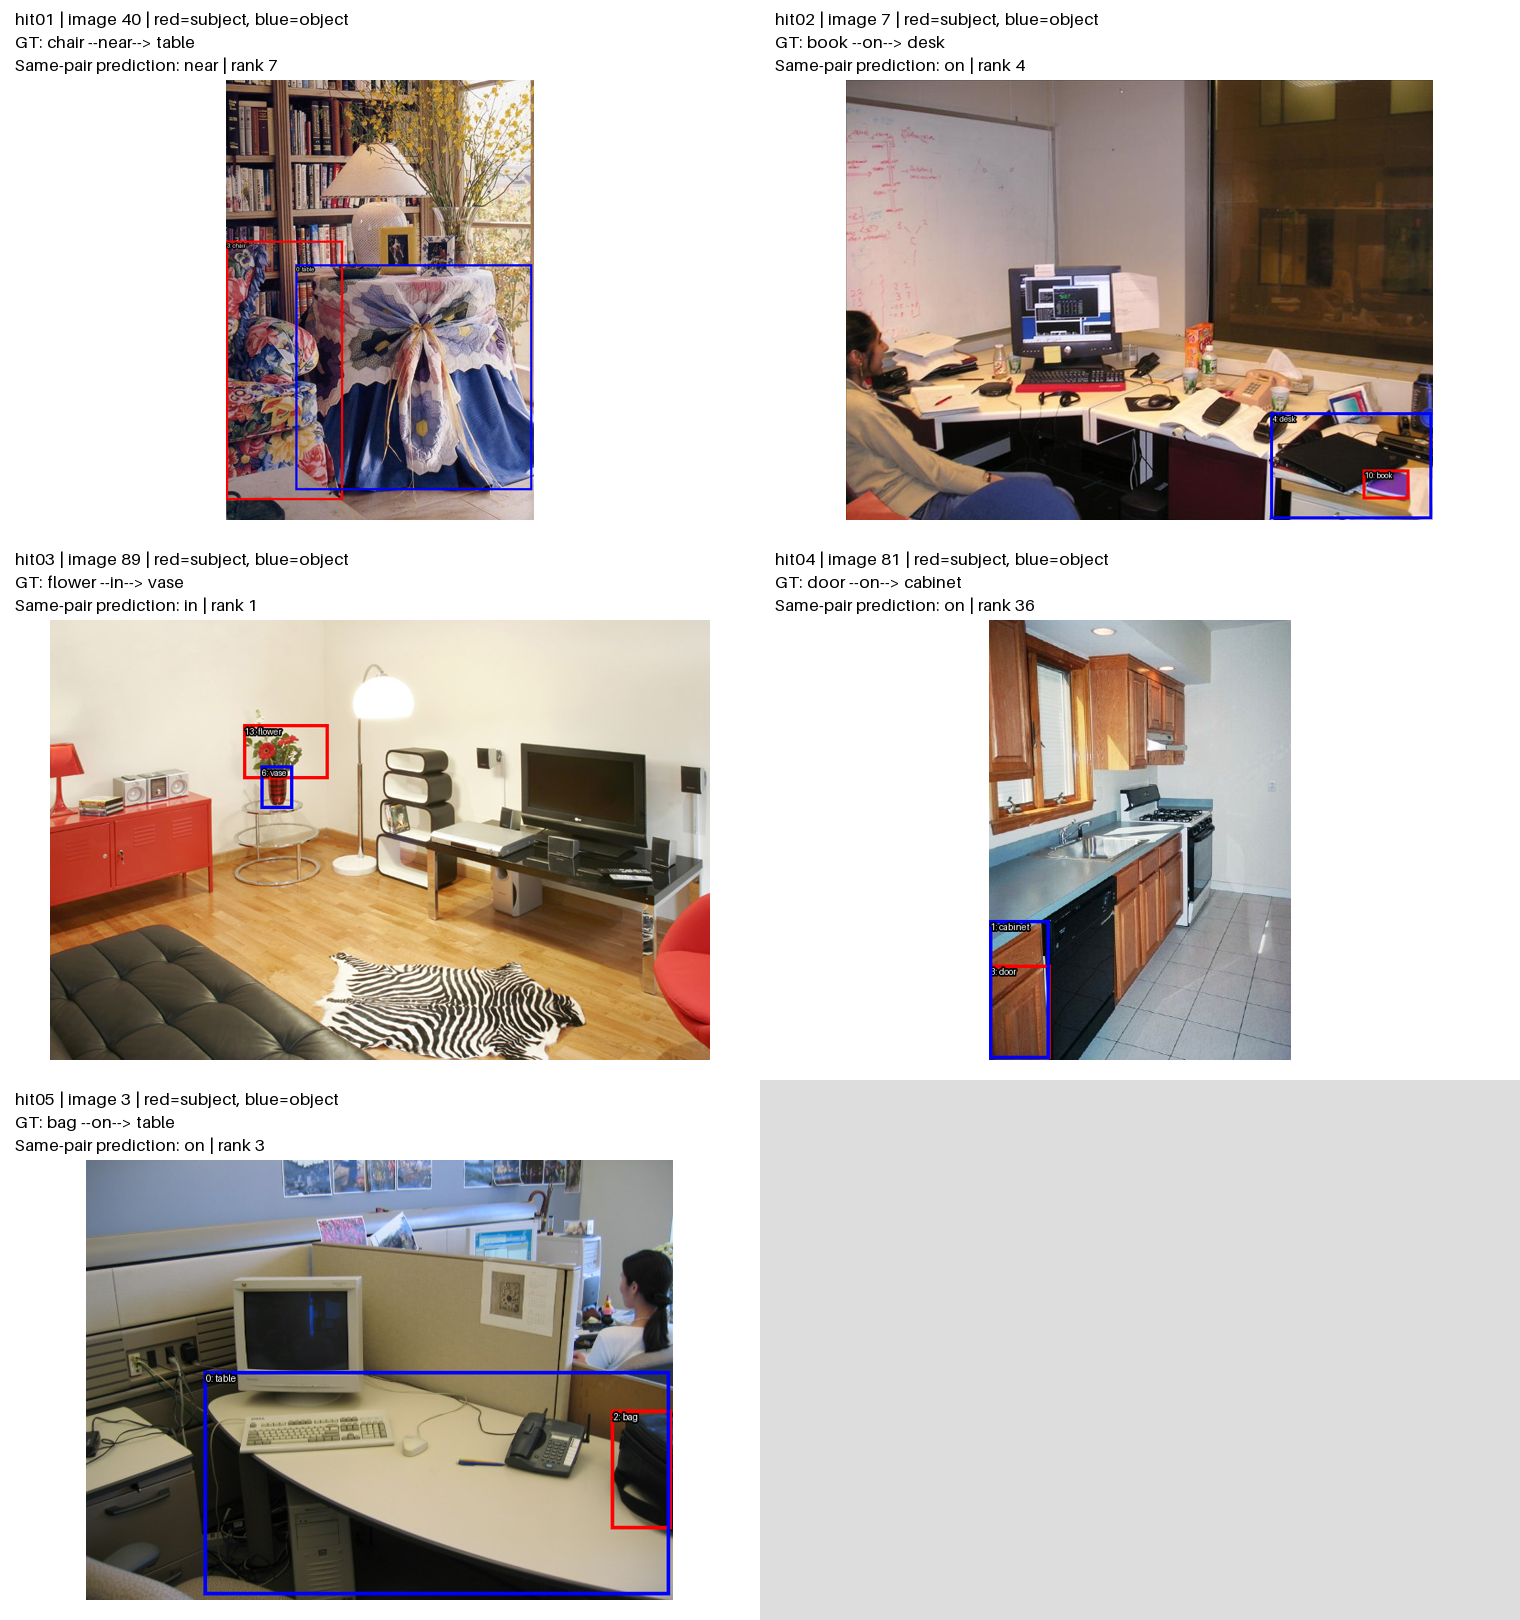
\includegraphics[width=.43\linewidth]{figures/vg-hit-contact-sheet.png}\hfill
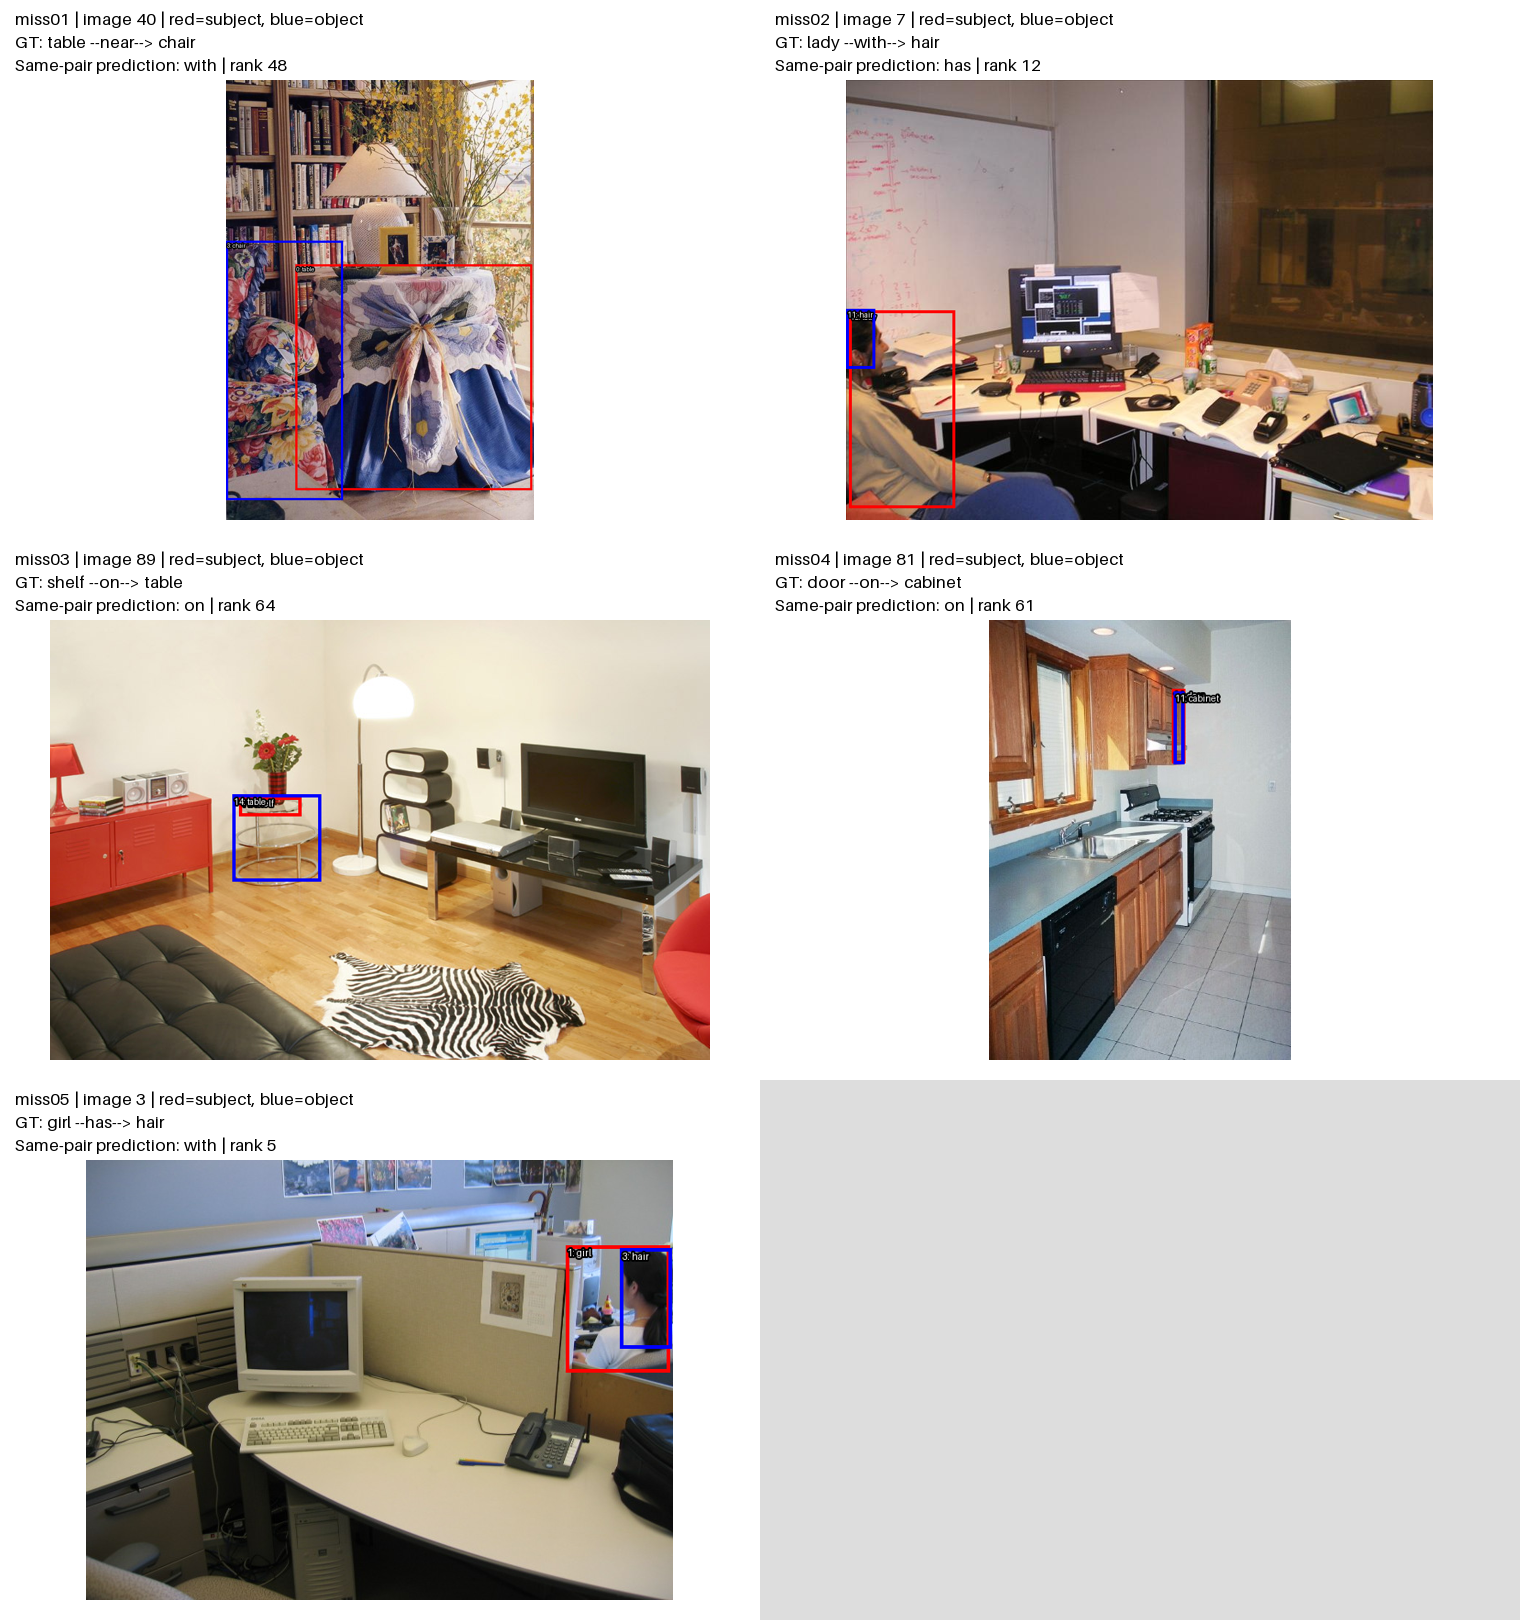
\includegraphics[width=.43\linewidth]{figures/vg-miss-contact-sheet.png}
\caption{Trái: H01--H05; phải: M01--M05, theo hàng từ trái sang phải.
Hộp đỏ là subject, xanh là object. Chi tiết GT và hạng nằm trong
bảng~\ref{tab:hits}--\ref{tab:misses}; ảnh gốc độ phân giải đầy đủ có trong artifact case.}
\end{figure*}
\srcnote{Nguồn: \path{reports/level1/submission/cases/}.
Đây là case validation đã có, không gắn lại nhãn thành case test.}


\section{Nhiệm vụ 2 -- Phương pháp mới và biến đổi đồ thị}
Nhiệm vụ 2 được tổ chức thành hai phần: Task A đáp ứng yêu cầu dataset thứ hai
và phương pháp từ năm 2023 trở lại đây; Task B học thao tác biến đổi đồ thị.
GQA thuộc Task A, không thuộc chương VG150.

\begin{figure*}[!t]\centering
\begin{tikzpicture}[font=\small,>=Latex,
b/.style={draw=inkblue,rounded corners,fill=mutedblue,align=center,minimum height=10mm,text width=63mm}]
\node[b,text width=55mm] (root) {Nhiệm vụ 2};
\node[b,anchor=north] (a) at (-3.8,-1.2) {Task A: dataset thứ hai + phương pháp mới\\Custom GQA: MLP/GAT/PE-Net/AlignG};
\node[b,anchor=north] (b) at (3.8,-1.2) {Task B: graph transformation\\MagicBrush $\to$ EMNLP 2020};
\draw[->] (root.south)--(a.north);
\draw[->] (root.south)--(b.north);
\end{tikzpicture}
\caption{Hai phần của Nhiệm vụ 2. EMNLP là dataset thay thế ở Task B.}
\end{figure*}

\subsection{Task A -- Custom GQA và phương pháp mới}
GQA có scene graph chuẩn hóa, phù hợp tái sử dụng pipeline PredCls với
đặc trưng CLIP đóng băng~\cite{hudson2019gqa}. Bản custom dùng 69.942 ảnh
train, 5.000 ảnh validation và 310 predicate foreground; đây không phải
benchmark GQA200. Các mô hình so sánh dùng cùng split và cùng evaluator nội bộ.

\begin{table}[!ht]\centering\small
\caption{Vai trò của từng cấu hình Task A.}\label{tab:gqamethod}
\begin{tabularx}{\linewidth}{@{}>{\raggedright\arraybackslash}p{26mm}X@{}}\toprule
Cấu hình & Thành phần được kiểm tra\\\midrule
MLP / GAT & Baseline phi đồ thị và message passing.\\
PE-CE & Nhánh prototype theo PE-Net, huấn luyện với cross-entropy.\\
PE-PL & Thêm prototype learning (PL).\\
PE-PLPR & Thêm prototype regularization (PR) vào PE-PL.\\
PE-PLPR + AlignG & Thêm cơ chế context/feedback vào baseline PE-PLPR trong matched ablation.\\
\bottomrule\end{tabularx}\end{table}

PE-Net~\cite{zheng2023penet} được adapted cho feature đã cache:
đặc trưng cặp thay cho union-box feature của detector gốc, có khởi tạo GloVe.
Nhánh AlignG~\cite{jung2026aligng} bổ sung prototype context và GRU feedback.
Do feature, label space và pipeline khác bản gốc, đây là \textbf{triển khai
adapted}, không phải reproduction hay so sánh trực tiếp với số trong paper.

\reporttodo{2A-1}{Bổ sung sơ đồ tensor của bản adapted, phương trình loss PL/PR,
trọng số từng loss và bảng ánh xạ module với paper từ source/config đã khóa.
Không điền công thức theo paper nếu code thực tế đã thay đổi.}
\reporttodo{2A-2}{Hoàn thiện data card custom GQA: cách lọc vocabulary, manifest chia ảnh,
và nguồn dữ liệu. Bảng test ở cuối mục dùng split riêng của đồ án.}
\srcnote{Nguồn: \path{docs/LEVEL2_METHOD_DECISION.md};
\path{reports/level2/gqa-full-v3-results-v1/README.md}.}


\subsection{Task A -- Bảng kết quả và matched ablation}
\begin{table*}[!t]\centering\small
\caption{Custom GQA validation; GC, mean $\pm$ sample std (\%), seed 42/123/3407.}\label{tab:gqa}
\begin{tabular}{@{}lrrrr@{}}\toprule
Model & R@50 & mR@50 & R@100 & mR@100\\\midrule
MLP & $76,66\pm0,59$ & $3,33\pm0,34$ & $87,24\pm0,40$ & $5,68\pm0,75$\\
GAT & $77,34\pm0,13$ & $3,10\pm0,10$ & $87,83\pm0,12$ & $4,84\pm0,22$\\
PE-CE & $78,07\pm0,27$ & $3,00\pm0,28$ & $88,39\pm0,25$ & $4,88\pm0,58$\\
PE-PL & $\mathbf{78,14\pm0,07}$ & $3,42\pm0,14$ & $\mathbf{88,51\pm0,05}$ & $5,61\pm0,48$\\
PE-PLPR & $77,97\pm0,07$ & $\mathbf{4,16\pm0,17}$ & $88,28\pm0,08$ & $\mathbf{7,13\pm0,31}$\\
\bottomrule\end{tabular}\end{table*}

R@50 quanh 77--78\% nhưng mR@50 chỉ 3--4\%: recall tổng thể che khuất chênh lệch
giữa predicate. PE-PLPR tăng 1,16 pp mR@50 so PE-CE, trong khi R@50
giảm 0,10 pp. GAT tăng R nhưng giảm mR so MLP, khác với xu hướng trên VG150.

\begin{table*}[!t]\centering\small
\caption{Matched ablation AlignG trên cùng custom GQA validation.}\label{tab:aligng}
\begin{tabular}{@{}lrrr@{}}\toprule
Model & GC R@50 & GC mR@50 & NG mR@50\\\midrule
PE-PLPR & $77,97\pm0,07$ & $4,16\pm0,17$ & $7,72\pm0,26$\\
PE-PLPR + AlignG & $77,95\pm0,16$ & $4,59\pm0,39$ & $9,12\pm1,11$\\
Delta từ mean hiển thị (pp) & $-0,02$ & +0,43 & +1,40\\
\bottomrule\end{tabular}\end{table*}

\begin{figure}[!ht]\centering
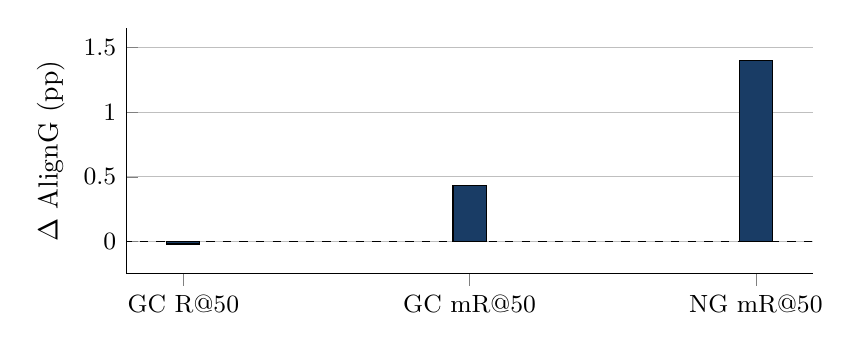
\begin{tikzpicture}
\begin{axis}[width=.85\linewidth,height=4.7cm,ybar,bar width=12pt,
ymin=-.25,ymax=1.65,xtick={1,2,3},
xticklabels={GC R@50,GC mR@50,NG mR@50},
ylabel={$\Delta$ AlignG (pp)},ymajorgrids,
tick label style={font=\small},axis x line*=bottom,axis y line*=left]
\addplot[fill=inkblue] coordinates {(1,-.02)(2,.43)(3,1.40)};
\draw[dashed] (axis cs:.5,0)--(axis cs:3.5,0);
\end{axis}\end{tikzpicture}
\caption{AlignG: thay đổi của mean hiển thị so với PE-PLPR. Không dùng ba metric
làm ba lần đo độc lập; độ biến động của từng model nằm trong bảng~\ref{tab:aligng}.}
\end{figure}

Matched ablation dùng cùng seed, batch 512, patience 15 và chọn checkpoint
theo validation GC mR@50. \textbf{PE-PLPR và AlignG cải thiện mean Recall,
không cải thiện đồng thời Recall tổng thể.}
\reporttodo{2A-3}{Thêm case đúng/sai có ảnh và graph, đối chiếu cùng cặp object
giữa PE-PLPR và AlignG. Chưa quy mức tăng mR cho một loại quan hệ cụ thể
khi chưa có phân tích per-predicate.}
\srcnote{Nguồn: \path{gqa-full-v3-results-v1/README.md};
\path{aligng-gqa-fast-v1-results-v1/summary.json} và \path{comparison.json}.
Delta tính từ số đầy đủ có thể lệch 0,01 pp so với hiệu hai mean đã làm tròn.}

\subsection{Test trên split riêng của đồ án}
Tập test gồm 10.696 ảnh từ phần validation chính thức của GQA, tách khỏi
5.000 ảnh validation nội bộ dùng để chọn checkpoint. Nhóm đã đối chiếu
27 lượt với danh sách checkpoint và cache đã khóa. Bảng~\ref{tab:gqatest}
dùng cùng ba seed 42, 123 và 3407 cho chín cấu hình.
\begin{table}[!ht]\centering\small
\caption{Custom GQA test, GC. Trung bình $\pm$ độ lệch chuẩn mẫu, đơn vị \%.}\label{tab:gqatest}
\begin{tabular}{@{}lrr@{}}\toprule
Mô hình & R@50 & mR@50\\\midrule
MLP & $76,86\pm0,45$ & $3,58\pm0,38$\\
GAT & $77,46\pm0,11$ & $2,97\pm0,24$\\
Edge-only & $77,79\pm0,02$ & $4,31\pm0,19$\\
GAT + KG & $77,42\pm0,04$ & $3,04\pm0,19$\\
PE-CE & $78,11\pm0,17$ & $2,93\pm0,16$\\
PE-PL & $78,21\pm0,09$ & $3,40\pm0,22$\\
PE-PLPR & $78,00\pm0,03$ & $4,07\pm0,20$\\
PE-CE + AlignG & $78,03\pm0,36$ & $3,52\pm0,32$\\
PE-PLPR + AlignG & $78,06\pm0,07$ & $4,62\pm0,57$\\
\bottomrule\end{tabular}\end{table}
\srcnote{Nguồn: \path{reports/level2/gqa-test-v1/summary.json} và
\path{completion-audit.json} của cùng đợt test.}


\subsection{Task B -- Yêu cầu gốc và thí nghiệm MagicBrush}
Yêu cầu gốc là xây ít nhất 300 cặp $(G_s,q,\Delta G)$ từ MagicBrush hoặc
InstructPix2Pix, kiểm tay ít nhất 20 mẫu và dự đoán sáu thao tác:
thêm/xóa/thay node, thêm/xóa/thay edge. Đầu ra không chỉ có loại thao tác;
cần đúng entity, endpoint và payload để áp dụng lên graph nguồn.

\begin{table}[!ht]\centering\small
\caption{Thiết lập MagicBrush và kết quả test (\%, ba seed).}\label{tab:magic}
\begin{tabularx}{\linewidth}{@{}Xrr@{}}\toprule
Chỉ số & MLP & GNN\\\midrule
Micro-F1 operation & $3,75\pm1,82$ & $7,34\pm1,50$\\
Exact target graph & 0 & 0\\
Số cặp train / val / test & 301 / 67 / 69 & 301 / 67 / 69\\
\bottomrule\end{tabularx}\end{table}

MagicBrush~\cite{zhang2023magicbrush} cung cấp ảnh nguồn, instruction và ảnh đích.
Graph sinh từ ảnh rồi căn chỉnh instance để lấy operation đích.
Bản v3 dùng các head dự đoán có cấu trúc: copy entity cũ, tối đa 12 slot node mới,
attention chọn endpoint và ràng buộc transaction. Hidden 192, dropout 0,1,
batch 16, AdamW $3\times10^{-4}$, weight decay $10^{-2}$, tối đa 200 epoch;
seed 42/123/3407, chọn checkpoint bằng validation operation-F1.

\begin{table*}[!t]\centering\small
\caption{Chẩn đoán MagicBrush. Mỗi hàng ghi rõ mẫu số và phạm vi.}\label{tab:magicdiag}
\begin{tabularx}{\linewidth}{@{}p{49mm}p{28mm}X@{}}\toprule
Quan sát & Giá trị / phạm vi & Hàm ý\\\midrule
Payload biểu diễn được & 154/219 operation val & Một phần target vượt vocabulary/representation.\\
Mẫu biểu diễn đầy đủ & 15/67 mẫu val & Biểu diễn từng operation chưa bảo đảm cả chương trình khả thi.\\
Đúng loại và entity & 37/118 dự đoán; GNN seed 42 val & Grounding còn sai trước khi xét payload.\\
Node mới đúng tên object & 2/42; chẩn đoán val & Open vocabulary là nút thắt.\\
Target không xác định duy nhất & 15/20 mẫu phân tích & Instruction không quyết định toàn bộ graph difference.\\
\bottomrule\end{tabularx}\end{table*}

GNN tăng 3,59 pp micro-F1 so MLP nhưng cả hai không khớp chính xác graph đích.
Điểm thấp không chỉ là thiếu năng lực message passing: target còn chứa sai số
extractor/alignment và thay đổi không được instruction chỉ định.
Phân tích 20 mẫu nêu trên chưa được coi là kiểm tay độc lập toàn bộ dữ liệu.

\reporttodo{2B-1}{Hoàn thiện bảng P/R/F1 của MagicBrush cho cả sáu operation
từ artifact v3, ghi support và tách loại không có GT khỏi F1 bằng 0.
Kèm 20 mẫu kiểm tay có ID, tiêu chí, người duyệt và kết luận độ tin cậy.}
\srcnote{Nguồn: \path{magicbrush-manual-experiment-v3/result-audit.json}
(mean/std test đã đối chiếu); \path{magicbrush-manual-v3-error-analysis-v1/README.md}.
Không ghép số chẩn đoán validation vào mẫu số test 69.}


\subsection{Task B -- Vì sao chuyển sang EMNLP 2020?}
\begin{table*}[!t]\centering\small
\caption{Phạm vi được cải thiện và phần chưa được giải quyết khi đổi dataset.}
\begin{tabularx}{\linewidth}{@{}X X X@{}}\toprule
Vấn đề MagicBrush & EMNLP giải quyết gì & EMNLP không giải quyết gì\\\midrule
Graph phải sinh từ ảnh & Có graph nguồn/đích sẵn & Không kiểm chứng pipeline từ ảnh.\\
Instance alignment nhiễu & Correspondence cấu trúc rõ hơn & Chưa chứng minh image-disjoint.\\
Target không duy nhất & Graph target xác định hơn & Graph nhỏ và đơn giản.\\
Open vocabulary lớn & Từ vựng khép kín hơn & Không đại diện đầy đủ scene graph ảnh thật.\\
\bottomrule\end{tabularx}\end{table*}

EMNLP 2020~\cite{he2020sgmod} là \textbf{dataset thay thế cho Task 2B},
dùng kiểm tra khả năng học operation với supervision có cấu trúc.
Kết quả này không xóa bỏ hoặc thay thế khó khăn đã ghi nhận trên MagicBrush.

\begin{table}[!ht]\centering\small
\caption{Thiết lập EMNLP 2020, phiên bản W\&B v4.}
\begin{tabularx}{\linewidth}{@{}p{24mm}X@{}}\toprule
Thành phần & Thiết lập\\\midrule
Dữ liệu & Train 29.868 / val 532 / test 530 mẫu.\\
Test subset & Từ 1.000 mẫu official: loại 468 source overlap train/val và 2 correspondence mơ hồ.\\
Representation & Graph gốc nhỏ (1--3 node), vô hướng, có attribute node; adapter tạo cạnh hai chiều.\\
Mô hình / tối ưu & Hidden 96; GNN 2 lớp; batch 128; AdamW $10^{-3}$, weight decay $10^{-2}$.\\
Chọn checkpoint & Validation token loss; tối đa 20 epoch, tối thiểu 6, patience 3; seed 42/43/44.\\
Theo dõi & Sáu run có W\&B; tổng 61 epoch, từng run dừng ở epoch 9--11.\\
\bottomrule\end{tabularx}\end{table}

Chia theo source fingerprint giảm trùng graph nhưng chưa chứng minh tách theo
ảnh gốc. Vocabulary chỉ xây từ train; 35/530 chương trình test có OOV vẫn được
giữ trong mẫu số. Ngưỡng exact tối đa do vocabulary là 93,40\%, không phải điểm
mô hình đạt được.

\reporttodo{2B-2}{Bổ sung sơ đồ encoder/decoder và loss của EMNLP v4 từ code đã khóa,
cách serialize operation và kiểm tra transaction. Không dùng mô tả các head
MagicBrush v3 thay cho kiến trúc EMNLP.}
\reporttodo{2B-3}{Hoàn thiện kiểm tay correspondence và instruction--target của EMNLP,
ví dụ graph trước/sau; xác minh nguồn ảnh và image-disjoint nếu metadata cho phép.
Ghi nhận việc trao đổi với giảng viên về thay đổi dataset.}


\subsection{Task B -- Kết quả EMNLP và phân tích theo operation}
\begin{table}[!ht]\centering\small
\caption{EMNLP test, 530 mẫu; mean $\pm$ sample std (\%), ba seed.}\label{tab:emnlp}
\begin{adjustbox}{max width=\linewidth}\begin{tabular}{@{}lrrrr@{}}\toprule
Model & Micro-F1 & Macro-F1 & Exact target & Valid transaction\\\midrule
MLP & $81,69\pm0,31$ & $54,25\pm0,51$ & $67,74\pm0,68$ & $95,60\pm0,29$\\
GNN & $82,44\pm0,39$ & $55,03\pm0,28$ & $68,55\pm0,22$ & $95,79\pm0,39$\\
\bottomrule\end{tabular}\end{adjustbox}\end{table}

\begin{table*}[!t]\centering\small
\caption{P/R/F1 theo operation trên EMNLP test; mean (\%). Support là số GT, không nhân ba seed.}\label{tab:operations}
\begin{tabular}{@{}lrrrrr@{}}\toprule
Operation & Support & MLP F1 & GNN P & GNN R & GNN F1\\\midrule
add\_node & 105 & 59,72 & 62,50 & 65,40 & 63,86\\
delete\_node & 363 & 97,10 & 97,53 & 97,98 & 97,76\\
replace\_node & 121 & 27,71 & 30,59 & 24,79 & 27,38\\
add\_edge & 210 & 43,86 & 42,64 & 44,60 & 43,56\\
delete\_edge & 728 & 97,10 & 97,53 & 97,76 & 97,64\\
replace\_edge & 6 & 0,00 & 0,00 & 0,00 & 0,00\\
\bottomrule\end{tabular}\end{table*}

GNN hơn MLP 0,75 pp micro-F1 nhưng chỉ hơn 0,78 pp macro-F1.
Deletion chiếm nhiều GT và đạt F1 gần 98\%, kéo micro-F1 lên;
replace-node chỉ 27,38\%, replace-edge có GT nhưng không có true positive.
Vì vậy micro-F1 82,44\% không có nghĩa cả sáu operation đều được học tốt.

\begin{table*}[!t]\centering\small
\caption{Đối chứng và lát cắt bổ sung trên cùng test.}
\begin{tabularx}{\linewidth}{@{}p{49mm}p{35mm}X@{}}\toprule
Đối chứng / lát cắt & Kết quả & Cách đọc\\\midrule
No-op & F1 0; exact 0; valid 100 & Hợp lệ cú pháp không đồng nghĩa đúng yêu cầu.\\
Nearest training program & F1 56,22; exact 33,77 & Baseline retrieval bằng CLIP instruction và pooled source.\\
GNN, simple exact & $24,79\pm1,65$ & 121 mẫu có đúng một GT operation; thấp hơn exact toàn tập.\\
MLP, simple exact & $25,34\pm1,91$ & GNN không thắng ở mọi lát cắt.\\
\bottomrule\end{tabularx}\end{table*}

Validation micro-F1 của MLP là 80,39\%, GNN 80,25\%: thứ hạng không giống test.
Bản v4 giữ kết quả test bằng v3 vì best-checkpoint tensor bằng nhau; đóng góp
của v4 là tracking/resume/early stopping, không phải accuracy gain.

\reporttodo{2B-4}{Chèn hình graph nguồn, instruction, operation GT/dự đoán và graph
sau áp dụng cho các case đúng/sai đã lưu ID/hash. Tách lỗi identity, payload,
loại thao tác và transaction; bổ sung xác nhận ngữ nghĩa bằng người.}
\srcnote{Nguồn: \path{emnlp2020-task-b-wandb-v4-test-v1/README.md},
\path{metrics.json}, \path{error-analysis.json}. Test này từng được xem ở v3;
v4 không chọn lại cấu hình theo kết quả test.}


\section{Nhiệm vụ 3 -- Đánh giá nhất quán ngữ nghĩa}
\subsection{Benchmark, mô hình và luồng đánh giá}
VN100 có 100 ảnh nguồn và 200 yêu cầu: mỗi ảnh có hai edit độc lập bắt đầu từ
ảnh gốc. Qwen-Image-2.1 sinh ảnh đích với BF16, 40 steps, batch 1, seed 42;
REACT++ pretrained sinh 100 graph nguồn và 200 graph đích~\cite{qwenimage21,reactplusplus}.
Không huấn luyện lại editor hoặc extractor.

\begin{figure*}[!t]\centering
\begin{tikzpicture}[font=\scriptsize,>=Latex,node distance=7mm and 5mm,
b/.style={draw=inkblue,fill=mutedblue,rounded corners,align=center,text width=31mm,minimum height=11mm}]
\node[b] (images) {100 ảnh nguồn\\200 instruction};
\node[b,right=of images] (edit) {Qwen-Image-2.1\\200 ảnh đích};
\node[b,right=of edit] (graphs) {REACT++\\graph nguồn/đích};
\node[b,right=of graphs] (score) {Alignment + scoring\\$E,P,G$};
\draw[->] (images)--(edit);\draw[->] (edit)--(graphs);\draw[->] (graphs)--(score);
\node[b,below=of edit] (human) {Nhãn tay\\fulfillment/preservation};
\node[b,below=of score] (eval) {Đánh giá tương quan\\cùng CLIPScore/$-$LPIPS};
\draw[->] (score)--(eval);\draw[->] (human)--(eval);
\end{tikzpicture}
\caption{Nhãn tay chỉ đi vào bước đánh giá tương quan. Scorer dùng grounding
instruction đã chuẩn bị, chưa nhận operation dự đoán từ Task 2.}
\end{figure*}

\begin{table}[!ht]\centering\small
\caption{Thiết lập alignment và scoring.}
\begin{tabularx}{\linewidth}{@{}p{24mm}X@{}}\toprule
Thành phần & Quy tắc\\\midrule
Cặp node ứng viên & Nhãn chuẩn hóa bằng nhau, IoU hộp ít nhất 0,3.\\
Matching & Hungarian: tối đa số cặp hợp lệ, sau đó tối đa tổng IoU.\\
Mơ hồ & Chênh IoU so với ứng viên cạnh tranh dưới 0,05.\\
Bằng chứng edit & Confidence ít nhất 0,4; IoU 0,5 để phát hiện khả năng relabel.\\
Add / remove / replace & Node mới đúng lớp và ROI / mất instance và giảm count / kết hợp xóa và thêm.\\
Abstention & Thiếu bằng chứng hoặc alignment mơ hồ: null, không tự gán 0.\\
\bottomrule\end{tabularx}\end{table}

Gọi $\mathcal C$ là tập kiểm tra nhị phân quan sát được của instruction,
$V^p,E^p$ là node/cạnh được bảo vệ sau khi loại phần được phép chỉnh sửa:
\[
E=\frac{1}{|\mathcal C|}\sum_{c\in\mathcal C}c,\qquad
D(A,B)=\frac{2|A\cap B|}{|A|+|B|},
\]
\[
P=\operatorname{mean}\{D(V_s^p,V_t^p),D(E_s^p,E_t^p)\}_{\mathrm{defined}},
\qquad G=E\,P.
\]
Các tập đích được đưa về hệ ID nguồn qua alignment; cạnh là triplet có hướng.
$E$ chỉ xác định khi mọi kiểm tra cần thiết xác định. Mười edit màu có
$E=G=\mathrm{null}$ vì graph không chứa màu; $P$ cấu trúc chỉ là chẩn đoán.
\reporttodo{3-1}{Hoàn thiện data card VN100, nguồn/giấy phép từng ảnh và minh chứng
được phép sử dụng. Thêm kiểm tay mẫu graph để đo độ tin cậy REACT++ trên benchmark.}


\subsection{Tương quan, error bar và coverage}
Nhãn tổng là AND của fulfillment và preservation: 175/200 cặp đạt, 25 không đạt.
Có 287 ô trống trên 144 cặp được chuẩn hóa thành đạt theo xác nhận của người duyệt;
đây là một phần protocol nhãn, không phải suy luận tự động từ ô trống.
Tập giao có đủ $G$ gồm 91 cặp thuộc 62 ảnh, với 82 đạt và 9 không đạt.

\begin{table}[!ht]\centering\small
\caption{Spearman với nhãn tổng trên cùng $N=91$; bootstrap 2.000 lượt theo cụm ảnh, seed 42.}\label{tab:corr}
\begin{adjustbox}{max width=\linewidth}\begin{tabular}{@{}lrc@{}}\toprule
Điểm & $\rho$ & Khoảng bootstrap 95\%\\\midrule
Graph $G$ & 0,1767 & $[-0,0304;\ 0,3571]$\\
CLIPScore & 0,0561 & $[-0,1245;\ 0,2233]$\\
$-\mathrm{LPIPS}$ & 0,1962 & $[-0,0178;\ 0,3908]$\\
\bottomrule\end{tabular}\end{adjustbox}\end{table}

\begin{figure}[!ht]\centering
\begin{tikzpicture}
\begin{axis}[width=.85\linewidth,height=4.6cm,xmin=-.18,xmax=.45,
xtick={-.1,0,.1,.2,.3,.4},xticklabel style={/pgf/number format/fixed},
ymin=.5,ymax=3.5,ytick={1,2,3},yticklabels={CLIPScore,Graph,$-\mathrm{LPIPS}$},
xlabel={Spearman $\rho$, khoảng bootstrap 95\%},
axis x line*=bottom,axis y line*=left,xmajorgrids]
\addplot+[only marks,color=inkblue,error bars/.cd,x dir=both,x explicit]
coordinates {(.0561,1) +=(.1672,0) -=(.1806,0)
(.1767,2) +=(.1804,0) -=(.2071,0)
(.1962,3) +=(.1946,0) -=(.2140,0)};
\draw[dashed] (axis cs:0,.5)--(axis cs:0,3.5);
\end{axis}\end{tikzpicture}
\caption{Cả ba khoảng đều chứa 0. Thứ tự point estimate chưa đủ để kết luận
một chỉ số tốt hơn chỉ số khác; cần xét phân phối chênh lệch ghép cặp.}
\end{figure}

CLIPScore dùng CLIP ViT-B/32 và $2,5\max(\cos(I_t,q),0)$ với text prefix
của pipeline~\cite{hessel2021clipscore}. LPIPS AlexNet đo khoảng cách ảnh
nguồn--đích~\cite{zhang2018lpips}; lấy dấu âm để điểm cao tương ứng gần nguồn.
LPIPS có thể thưởng cho giữ nguyên ảnh dù chưa làm đúng yêu cầu.
Riêng $E$ tương quan 0,2008 với fulfillment ($N=162$);
$P$ tương quan 0,0302 với preservation ($N=109$).

\begin{table}[!ht]\centering\small
\caption{Coverage và tương quan theo loại edit. Không gán abstention thành lỗi ảnh.}\label{tab:coverage}
\begin{adjustbox}{max width=\linewidth}\begin{tabular}{@{}lrrrr@{}}\toprule
Loại & Tổng cặp & Có $G$ & Coverage (\%) & $\rho_G$\\\midrule
Thêm object & 106 & 60 & 56,6 & 0,0753\\
Xóa object & 66 & 23 & 34,8 & 0,1271\\
Thay object & 18 & 8 & 44,4 & 0,2474\\
Đổi màu & 10 & 0 & 0,0 & Không xác định\\\midrule
Tổng & 200 & 91 & 45,5 & 0,1767\\
\bottomrule\end{tabular}\end{adjustbox}\end{table}
\reporttodo{3-2}{Đính kèm provenance xác nhận nhãn và quy tắc chuẩn hóa ô trống.
Bổ sung người duyệt thứ hai/agreement nếu thực hiện; hiện chỉ có một người duyệt.
Giữ nguyên kết quả hiện có, không điền nhãn mới theo điểm model.}


\subsection{Failure taxonomy và mười ca bất đồng}
Các ca được chọn theo chênh lệch thứ hạng giữa graph và baseline ảnh trên tập
giao; tất cả thuộc nhóm thêm object. Đây là case study có chủ đích,
không đại diện cho tần suất lỗi của 200 edit.

\begin{table}[!ht]\centering\small
\caption{Mười ca bất đồng đã phân tích; cần bổ sung ảnh/graph minh họa.}\label{tab:cases3}
\begin{tabularx}{\linewidth}{@{}l p{29mm}X@{}}\toprule
ID & Yêu cầu & Chẩn đoán\\\midrule
58 & Thêm thuyền buồm & $G=1$; CLIP crop cắt thuyền ở bên trái.\\
69 & Thêm thuyền chèo & $G=1$, LPIPS cao; CLIP thấp, nguyên nhân chưa xác định.\\
178 & Thêm chim trên đá & Chim bị extractor nhận thành person; $G=0$.\\
168 & Thêm mèo dưới cây & $G=1$ dù nền/cây bị đổi; graph bỏ sót lỗi bảo toàn.\\
22 & Thêm chậu cây & Tủ vẫn còn nhưng mất refrigerator detection; $G=0,2$.\\
188 & Thêm chim bên chùa & Chim sai vị trí; $G=0$ nhưng do thiếu detection, không phải hiểu đúng vị trí.\\
160 & Thêm chim trên đá & Có bird nhưng tâm hộp ngoài ROI cứng; $G=0$.\\
187 & Thêm chó bên thác & $E=1$, $P$ giảm do detection nền thay đổi.\\
198 & Thêm chim bên ao & Graph phản ánh lan can thêm ngoài mục tiêu.\\
48 & Thêm ghế gỗ & $G=0,875$; CLIP thấp dù crop còn chứa ghế.\\
\bottomrule\end{tabularx}\end{table}

\begin{table}[!ht]\centering\small
\caption{Phân tầng lỗi để tránh quy mọi lỗi cho scorer.}
\begin{tabularx}{\linewidth}{@{}p{18mm}X p{15mm}@{}}\toprule
Tầng & Cơ chế & Case minh họa\\\midrule
Extractor & Bỏ sót hoặc nhầm nhãn object trước khi matching & 178, 22, 187\\
Grounding / alignment & Ràng buộc ROI cứng hoặc correspondence không chắc chắn & 160, 188\\
Biểu diễn & Graph không mã hóa đủ màu, texture, thay đổi nền & 168; edit màu\\
Baseline ảnh & Crop hoặc embedding không phản ánh đúng object được thêm & 58, 48\\
Chưa giải thích & Chênh lệch score chưa có nguyên nhân được xác minh & 69\\
\bottomrule\end{tabularx}\end{table}

\reporttodo{3-3}{Chèn ảnh nguồn/đích thật và graph overlay cho 10 ID trên,
kèm instruction, nhãn tay, $E/P/G$, CLIPScore và LPIPS. Ưu tiên panel 178
(extractor), 168 (bảo toàn), 160 (ROI) và 58 (crop) trong thân bài;
các panel còn lại có thể đặt ở phụ lục artifact.}
\reporttodo{3-4}{Bổ sung bảng số lượng abstention theo reason code, phân biệt
một mẫu có nhiều lý do với lý do chính. Không suy tần suất từ 10 case đã chọn.}

\textbf{Kết luận Nhiệm vụ 3.} Graph score giúp truy nguyên lỗi khi graph đáng tin,
nhưng coverage 45,5\%, tương quan yếu và thiếu thuộc tính chưa cho phép thay thế
human review. Bootstrap theo ảnh xử lý sự phụ thuộc của hai edit cùng nguồn;
không khắc phục selection bias do 109 abstention hoặc hạn chế một seed sinh ảnh.
\srcnote{Nguồn: \path{docs/LEVEL3_RESULTS_V1.md},
\path{LEVEL3_EVALUATION.md}, \path{LEVEL3_PIPELINE.md};
\path{configs/level3/evaluation200-v1.json}.}

\section{Mở rộng sang video trên PVSG}
\subsection{Từ một cạnh trong ảnh đến một quan hệ có thời hạn}
Ở thiết lập PredCls trên ảnh tĩnh, mô hình có thể dự đoán một quan hệ cho cặp
đối tượng từ một lần quan sát. Trong video, hai đối tượng có thể xuất hiện cùng
nhau lâu hơn hành động liên kết chúng. Chẳng hạn, người và chiếc cốc có thể
cùng ở trong khung hình cả trước khi người cầm cốc và sau khi đặt cốc xuống.
Đầu ra vì thế gồm ID chủ thể $s$, predicate $p$, ID đối tượng $o$ và tập frame
$A_{spo}$ trên đó quan hệ có hiệu lực. Một bộ ba có thể có nhiều đoạn rời nhau.
Hai cặp có thứ tự $(s,o)$ và $(o,s)$ được chấm riêng.

PVSG tách việc tìm và theo dõi vùng đối tượng khỏi việc tìm quan hệ trên
các track~\cite{yang2023pvsg}. Thực nghiệm này cấp mask, nhãn lớp và ID chuẩn
của đối tượng ở từng frame. ID nối các quan sát của cùng một đối tượng qua
thời gian. Mô hình phải tự chọn cặp, predicate và khoảng thời gian. Thiết lập
này cho phép quy khác biệt giữa các cấu hình cho phần dự đoán quan hệ khi đầu
vào đối tượng như nhau. Phạm vi khác với kiểm tra bảo toàn nội dung sau khi
chỉnh sửa video trên DAVIS hoặc YouTube-VOS được gợi ý trong đề.

\subsection{Dữ liệu, căn chỉnh và biểu diễn}
Bản PVSG phát hành gồm 400 video tại 5 frame/giây với 149.488 frame chú thích,
126 lớp đối tượng và 57 predicate. Ba nguồn là VidOR (289 video), Ego4D (56)
và EPIC-Kitchens (55). Nhóm giữ danh sách 338 video train và 62 video test
của bản phát hành. Tập train được chia thành 287 video fit và 51 video
validation. Việc chia theo video giữ các cửa sổ chồng lấn của một video trong
cùng một tập. Có bốn nhóm ID nguồn Ego4D xuất hiện ở cả hai phía của split phát
hành. Vì vậy độ độc lập theo cảnh quay gốc còn là một giới hạn.

Mask xác định trục thời gian và vùng nhìn thấy của mỗi track. Kiểm tra media phát
hiện bốn frame RGB thiếu; tại những vị trí này vẫn giữ thông tin hình học và
cờ chỉ báo thiếu đặc trưng thị giác. Với nhãn quan hệ, nhóm lấy giao thời gian
chú thích với các frame hai track cùng nhìn thấy. Các nhãn ngoài từ vựng,
tham chiếu track sai và đoạn rỗng sau phép giao được ghi vào nhật ký xử lý.
Cách làm này giữ nguyên danh sách video và cho mọi mô hình cùng một tập đích.
CLIP ViT-B/32~\cite{radford2021clip} đóng băng trích vector ảnh 512 chiều; cache dùng chung cho cả
400 video. Nhờ vậy có thể thay relation head mà vẫn dùng đúng đặc trưng
của cùng một vùng trên cùng một frame.

\subsection{Đồ thị và các mô hình đối chứng}
Một đỉnh biểu diễn một đối tượng nhìn thấy tại một frame. Cạnh không gian
cho phép trao đổi thông tin giữa đối tượng cùng frame. Cạnh thời gian nối hai
quan sát liền kề của cùng track. Tập cặp cần dự đoán gồm mọi cặp có hướng,
khác ID, có ít nhất một frame đồng hiện. Tập cặp này vẫn giữ nguyên khi bỏ
cạnh truyền thông điệp trong mô hình. Nhờ đó ablation đo ảnh hưởng của ngữ
cảnh mà không làm bài toán dễ đi bằng cách loại ứng viên.

MLP mã hóa đối tượng và chấm từng cặp ở từng frame. Static GAT cho phép các
đỉnh lấy ngữ cảnh trong một frame trước khi chấm cặp. ST-GAT thêm ngữ cảnh
trên track; hai lớp thời gian cho trường tiếp nhận tối đa năm frame.
Ba biến thể lần lượt bỏ cạnh thời gian, bỏ cạnh không gian và bỏ cả hai loại
cạnh giữa các đỉnh. Cả ba giữ self-loop và cùng kiến trúc ST-GAT. Do đó Static
GAT và ST-GAT bỏ cạnh thời gian vẫn là hai cấu hình riêng.

Mô hình Temporal Conv xử lý chuỗi đặc trưng của cùng một cặp đối tượng. Khi một
đối tượng khuất, chuỗi được tách tại chỗ mất đồng hiện. Conv kernel 5, ba lớp
chuyển thể thiết kế trong mục 5.2 của bài PVSG. Nhóm dùng projection cặp và
đầu ra đa nhãn chung thay cho các đầu ra riêng của OpenPVSG. Conv kernel 3,
hai lớp là đối chứng bổ sung. Trường tiếp nhận tối đa tương ứng là 13 và 5 frame.
Trong bài CVPR, segmentation và tracking cung cấp track dự đoán, nên điểm
end-to-end còn phản ánh cả lỗi mask, lớp và liên kết ID. Bảng của nhóm chỉ so
sánh trực tiếp tám cấu hình dùng cùng GT track.

\subsection{Từ điểm từng frame đến khoảng dự đoán}
Với mỗi cặp và frame hợp lệ, mô hình xuất 57 logits; masked binary
cross-entropy cho phép nhiều quan hệ đồng thời. Khi đánh giá, cửa sổ dài 64
frame, bước trượt 32. Với frame thuộc nhiều cửa sổ, lấy trung bình logits
trước sigmoid rồi chọn các frame có xác suất ít nhất 0,5. Mỗi đoạn frame liên
tiếp tạo một interval với hai đầu mút tính cả. Điểm xếp hạng của bộ ba là xác
suất trung bình trên các frame đã chọn. Cách này trả về nhiều khoảng cho cùng
bộ ba và xếp hạng sau khi đã ghép toàn bộ video.

Gọi $A$ là tập frame dự đoán và $B$ là tập frame chuẩn của cùng bộ ba.
Khi đó $\mathrm{tIoU}=|A\cap B|/|A\cup B|$. Ví dụ, nếu nhãn gồm các
frame 10--14 và dự đoán gồm các frame 12--16, phần giao có ba frame và
phần hợp có bảy; bộ ba đúng vẫn bị tính trượt ở ngưỡng 0,5. Khi $B$ có hai
đoạn rời, phép tính trên tập frame giữ được khoảng trống giữa hai đoạn.

Mỗi video lấy tối đa 50 bộ ba có điểm cao nhất. Một lượt trúng cần khớp
đúng thứ tự hai track, predicate và đạt tIoU ít nhất 0,5. R@50 lấy tổng
số trúng chia cho 931 bộ ba chuẩn trên 62 video. mR@50 tính recall riêng
từng lớp rồi lấy trung bình trên 54 lớp có mặt trong test. Cách gộp này khác
với trung bình trên từng ảnh trong protocol VG150.

\subsection{Huấn luyện và chọn checkpoint}
Mỗi cấu hình chạy ba seed 17, 42 và 2026 với batch 32, tối đa 150 epoch
và patience 15. Tiêu chí chọn là mR@50 validation, hòa thì xét R@50 rồi
lấy epoch sớm hơn. Sau khi xem validation và trước khi chấm test, nhóm
áp dụng cùng một điều kiện kiểm tra hội tụ muộn cho toàn bộ 24 cặp mô hình/seed.
Nếu lượt gốc dừng ở epoch 16 với cả hai recall validation bằng 0, huấn
luyện lại từ đầu với cùng seed và chỉ cho phép dừng từ epoch 50.
Bảng~\ref{tab:pvsg} gồm 17 lượt gốc và 7 lượt huấn luyện lại; mỗi seed
đóng góp đúng một giá trị. Cách chọn bảo đảm cùng tiêu chí giữa các seed
trong khi cho phép chi phí huấn luyện thực tế khác nhau. Bảy so sánh từng
cặp nằm ở Phụ lục~\ref{app:late}.

\begin{table}[!ht]\centering
\caption{PVSG test trên track chuẩn. Bảng chính có tính hội tụ muộn;
trung bình $\pm$ độ lệch chuẩn mẫu của ba seed, đơn vị \%.}\label{tab:pvsg}
\small\setlength{\tabcolsep}{3pt}
\begin{tabular}{@{}lrr@{}}\toprule
Mô hình & R@50 & mR@50\\\midrule
MLP & $3,80\pm0,43$ & $1,62\pm0,12$\\
Static GAT & $3,80\pm0,65$ & $1,68\pm0,17$\\
ST-GAT & $4,98\pm0,27$ & $\mathbf{2,38\pm0,54}$\\
ST-GAT bỏ cạnh thời gian & $3,58\pm1,35$ & $1,28\pm0,75$\\
ST-GAT bỏ cạnh không gian & $3,47\pm1,20$ & $1,07\pm0,70$\\
ST-GAT chỉ giữ self-loop & $3,62\pm0,16$ & $1,51\pm0,04$\\
Conv kernel 3, hai lớp & $6,77\pm0,65$ & $1,29\pm0,26$\\
Conv kernel 5, ba lớp & $\mathbf{8,63\pm0,61}$ & $1,25\pm0,25$\\
\bottomrule\end{tabular}
\end{table}

\subsection{Recall tổng, recall theo lớp và sai số thời gian}
Conv kernel 5 thu hồi nhiều bộ ba nhất; recall theo nguồn Ego4D,
EPIC-Kitchens và VidOR lần lượt là 11,72\%, 10,67\% và 7,18\%. Khi xếp 57
predicate theo tần suất trên tập fit và chia đều thành ba nhóm, mR@50 của
Conv kernel 5 lần lượt là 3,56\%, 0,00\% và 0,00\% từ phổ biến đến hiếm.
Một mô hình tập trung vào lớp phổ biến vì thế có thể tăng R@50 dù nhiều lớp
chưa có lượt trúng. ST-GAT đầy đủ đạt mR@50 cao nhất và có mean cao hơn cả
ba ablation cạnh. Với ba seed và độ phân tán quan sát được, đây là nhận xét
về các lượt đã đo. Hai Conv khác cả độ sâu lẫn số tham số; mức tăng R@50
của Conv kernel 5 chưa tách riêng được tác dụng của cửa sổ ngữ cảnh.

Ở Static GAT seed 17, bộ ba $(8,20,4)$ trong video \path{0004_11566980553}
được xếp trong top 50 nhưng đạt tIoU 0,289. Ở video
\path{0039_6951351121}, bộ ba $(14,43,3)$ có tIoU đúng bằng 0,50 và được
tính trúng. Hình~\ref{fig:timeline} đối chiếu một số tập frame chuẩn và dự
đoán. Cả hai ví dụ cho thấy phân tích chỉ ở mức tên quan hệ dễ bỏ qua sai số
định vị thời gian.


\section{Đối chiếu đề bài và hạn chế}
\begin{table*}[!t]\centering\small
\caption{Trạng thái theo đúng ba nhiệm vụ của đề bài.}\label{tab:compliance}
\begin{tabularx}{\linewidth}{@{}p{35mm}p{43mm}X@{}}\toprule
Phần & Trạng thái & Hạn chế / bằng chứng còn thiếu\\\midrule
Nhiệm vụ 1 -- VG150 & Đủ 54 kết quả test; long-tail 54 và zero-shot 9 checkpoint & Bộ hit/miss validation chưa thay thế kiểm tay 5 sai ngữ nghĩa kèm ảnh.\\
Nhiệm vụ 2A -- GQA & Có baseline, PE-Net và AlignG adapted & Có validation và test nội bộ, khác GQA200; TODO 2A-1--3.\\
Nhiệm vụ 2B -- MagicBrush & 437 cặp, có model và kết quả & Supervision yếu, exact 0; hoàn thiện kiểm tay và bảng operation, TODO 2B-1.\\
Nhiệm vụ 2B -- EMNLP & Đã đánh giá dataset thay thế trên test & Chưa chứng minh image-disjoint; cần giải trình và kiểm tay, TODO 2B-2--4.\\
Nhiệm vụ 3 -- VN100 & Đủ quy mô 100 ảnh/200 yêu cầu và so sánh baseline & Graph coverage 45,5\%; thiếu panel minh họa và audit, TODO 3-1--4.\\
Data card / license & Chưa hoàn tất & Bằng chứng nguồn và quyền sử dụng ảnh phải bổ sung trước nộp.\\
Đóng gói / demo & Chưa chốt bản nộp & Cần xác nhận đóng góp, khai báo công cụ/mã nguồn dùng lại, demo và liên kết artifact.\\
\bottomrule\end{tabularx}\end{table*}

\subsection{Giới hạn của kết luận}
\textbf{Protocol.} Chỉ so sánh số khi cùng dataset, split, evaluator và cohort.
Mean/std ba seed đo biến động run, không phải bằng chứng có ý nghĩa thống kê.
Không đồng nhất mR, zero-shot recall, operation-F1 và Spearman.

\textbf{Dữ liệu.} KG ngoài chỉ bổ sung tri thức; không chứng minh object/quan hệ
chưa từng xuất hiện trong pretraining. Custom GQA là nhánh adapted;
EMNLP kiểm tra supervision cấu trúc trên graph nhỏ. Đổi dataset không giải quyết
chất lượng graph sinh từ ảnh.

\textbf{Tích hợp.} Các mô-đun hiện được đánh giá riêng. Scorer Nhiệm vụ 3 dùng
grounding chuẩn bị sẵn, không dùng operation dự đoán của Task 2; chưa có bằng chứng
về chất lượng chuỗi end-to-end. Notebook minh họa là hạng mục riêng cần hoàn thiện.

\subsection{Artifact và khả năng truy vết}
Bản báo cáo dùng thêm các kết quả test mới, không còn gắn toàn bộ số liệu với
một commit cũ. Hai đợt chấm test VG150 có danh sách mã nguồn và checkpoint riêng. Với PVSG, danh sách 31 checkpoint và 62 ID test được khóa trước khi chấm. \path{SOURCE_MAP.md} liệt kê đường
dẫn tới nguồn của từng nhóm bảng; \path{TODO.md} tập hợp phần cần điền tiếp.
Không sửa source/manifest/config của thí nghiệm cũ để làm khớp nội dung báo cáo.

\subsection{Đóng góp và khai báo công cụ}
Danh sách tác giả theo hồ sơ của nhóm được ghi ở Bảng~\ref{tab:credits}.
Phân công chi tiết và minh chứng commit cần từng thành viên xác nhận trước khi nộp.
\begin{table}[!ht]\centering\small
\caption{Thành viên và trạng thái xác nhận đóng góp.}\label{tab:credits}
\begin{tabular}{@{}lll@{}}\toprule
Mã học viên & Thành viên & Phân công\\\midrule
24C15002 & Hồ Thanh Bình & Chờ xác nhận\\
24C15026 & Dương Thuỷ Tiên & Chờ xác nhận\\
25C15039 & Bùi Mạnh Hùng & Chờ xác nhận\\
25C15046 & Nguyễn Đăng Khoa & Chờ xác nhận\\
25C15062 & Nguyễn Đăng Thới Toàn & Chờ xác nhận\\
\bottomrule\end{tabular}
\end{table}
Các thành phần dùng lại gồm bộ trích CLIP, các mô hình sinh ảnh và trích
đồ thị đã dẫn ở Nhiệm vụ 3, cùng thiết kế Temporal Conv của PVSG.
Phần video thay đầu vào bằng track chuẩn và thay đầu ra bằng điểm đa nhãn
theo frame để dùng chung loss, decoder và evaluator. Công cụ AI (Codex)
hỗ trợ chuyển nguồn LaTeX sang IEEE Conference, đối chiếu số liệu và kiểm
tra bản biên dịch. Phạm vi các công cụ khác do từng thành viên sử dụng
cần được nhóm xác nhận.

\subsection{Kết luận}
Trên VG150 test, bằng chứng rõ nhất là cải thiện mR từ GAT và adjusted loss;
tác động nội dung KG chưa ổn định trước shuffled control. Trên Task 2,
PE-PLPR/AlignG tăng mR ở custom GQA, còn khoảng cách MagicBrush--EMNLP
cho thấy chất lượng supervision là nút thắt của graph transformation.
Trên Task 3, graph score có khả năng chẩn đoán nhưng chưa vượt baseline ảnh
và chỉ đánh giá được 45,5\% cặp. Những kết luận này được giới hạn theo
split và bằng chứng đã đo. Trên PVSG, việc cung cấp track chuẩn tách được
bài toán nhận biết quan hệ khỏi bài toán tìm đối tượng. Conv kernel 5 đạt recall
tổng cao nhất, trong khi ST-GAT đạt recall trung bình theo lớp cao nhất khi áp dụng
quy tắc kiểm tra hội tụ muộn cho mọi seed.

\printbibliography[title={Tài liệu tham khảo}]
\onecolumn
\appendices
\section{Bảy lượt kiểm tra hội tụ muộn trên PVSG}\label{app:late}
Mỗi hàng đối chiếu hai lượt có cùng mô hình và seed. Lượt gốc có cả hai
recall test bằng 0. Khi hoãn thời điểm được phép dừng, cả bảy lượt vẫn có
recall validation bằng 0 đến hết epoch 16. Lượt trúng validation đầu tiên
xuất hiện trong khoảng epoch 17--20. Bảng~\ref{tab:late} ghi kết quả test
của checkpoint chọn bằng validation trong mỗi lượt kiểm tra bổ sung.
\begin{table}[H]\centering\small
\caption{Kết quả từng seed khi hoãn early stopping. Đơn vị \%.}\label{tab:late}
\begin{tabular}{@{}lrrr@{}}\toprule
Cấu hình ST-GAT & Seed & R@50 & mR@50\\\midrule
Đầy đủ & 17 & 5,26 & 1,87\\
Đầy đủ & 2026 & 4,73 & 2,31\\
Bỏ cạnh thời gian & 17 & 4,83 & 1,77\\
Bỏ cạnh thời gian & 2026 & 2,15 & 0,41\\
Chỉ giữ self-loop & 17 & 3,76 & 1,52\\
Chỉ giữ self-loop & 42 & 3,65 & 1,55\\
Chỉ giữ self-loop & 2026 & 3,44 & 1,46\\
\bottomrule\end{tabular}
\end{table}
\section{Ví dụ thời gian trên track chuẩn}
\begin{figure}[H]\centering
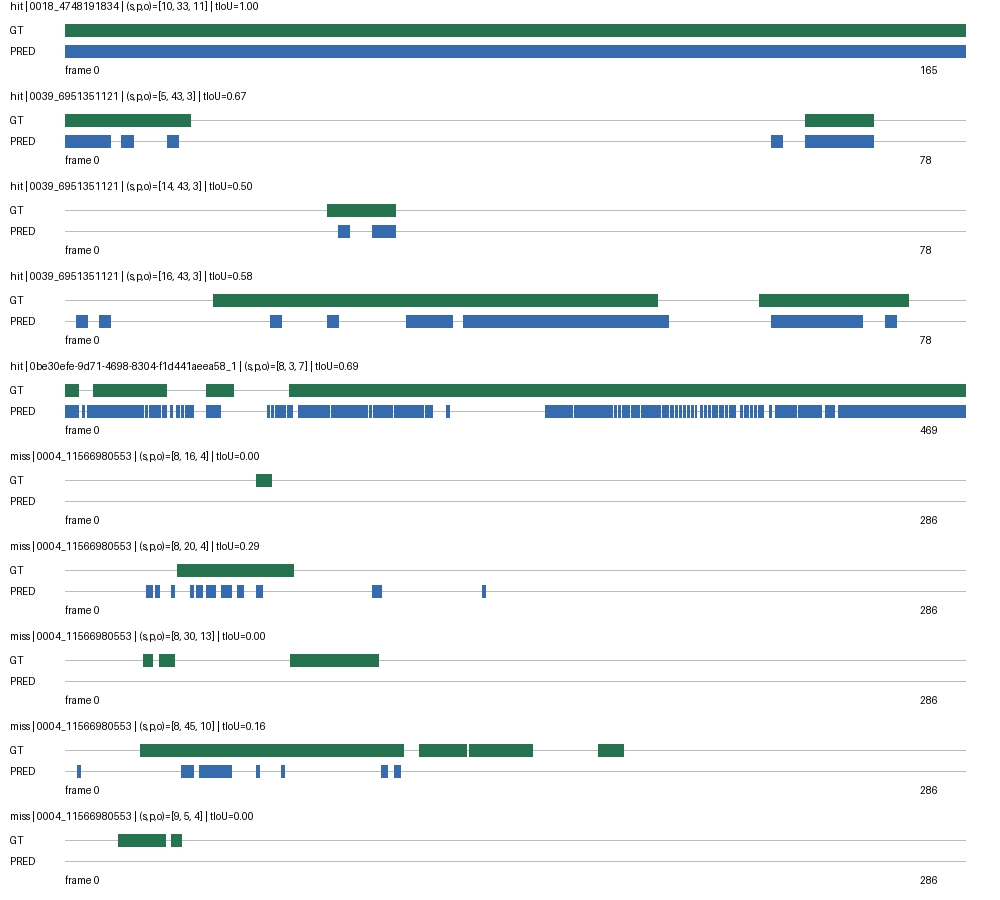
\includegraphics[width=.80\linewidth]{case_timelines.png}
\caption{Đoạn chuẩn (GT, xanh lá) và đoạn dự đoán (PRED, xanh dương) của Static GAT seed 17. Mười trường
hợp được lấy theo thứ tự video và bộ ba trong mỗi nhóm trúng hoặc bỏ sót.
Mỗi hàng có trục frame riêng.}\label{fig:timeline}
\end{figure}

\end{document}
